\chapter{The First Width of Planar Domains}
\label{ch:3}

As stated in the introduction, we focus on the \emph{first width} for planar domains, defined in direct analogy to the second eigenvalue of a linear operator via the Courant--Fischer characterisation (\ref{CourantFischer}), but for the $\mathbf{Length}$ functional. The mountain pass framework that underlies the study in this chapter is: the \textbf{space of objects} is a class of smooth curves in the domain; the \textbf{admissible families} of these curves are $1$-parameter \emph{sweep--outs}; the \textbf{functional} is the length of curves in these families. While higher $p$-widths - analogous to higher eigenvalues - are well defined, our present aim is to focus on the case of the first width, which is already complex enough. Our main goal is to present a novel proof of the characterisation of the first width for planar convex polygons. The first width, $\omega_1(\Omega)$, is the largest number $L$ such that every $1$-parameter sweep-out contains a curve of length at least $L$. It plays the same role for curves in $\Omega$ as the second eigenvalue for a matrix: the minimal unavoidable length encountered when sweeping the domain with one degree of freedom. We define sweep--outs precisely and present a new proof that, for convex polygons, the first width coincides with the classical minimal width. Finally, we discuss how this viewpoint may extend to higher dimensions. This last part is offered not as a proof, but rather an outlook towards computing widths of convex, compact domains in more general settings.

\section{Sweep-outs}
We restrict our attention to simply-connected, compact domains $\Omega\subset\mathbb{R}^2$. Fix the reference $1$-parameter family,
\begin{equation}
\gamma^{*}_{t}\;=\;D^{2}\cap\{\,y=t\,\}, \qquad t\in[-1,1],
\end{equation}
namely the set of horizontal chords on the unit disc.
In this dissertation we adopt a simpler notion of sweep-outs, narrower than the one used in the standard treatments by authors such as Guth (\cite{Guth07}), Guaraco (\cite{{Guaraco18}}), Chodosh and Cholsaipant (\cite{Chodosh25}). We define a ($1$-parameter) sweep-out of $\Omega$ as any family of curves obtained from $\{\gamma^{*}_{t}\}$ by a “nice”, smooth deformation to the push--forward of the reference family, under a continuous map from the disc to the domain. \\
For the construction of diffeomorphisms with “nice” properties, we note some key definitions from Hatcher \cite{Hatcher02} and Hirsch \cite{Hirsch76}. The essential ideas of “deformation without tearing” and winding numbers are stated here; further background and related remarks appear in Appendix (\ref{appendix-2}).

\begin{definition}[Isotopy (see \ref{def:isotopy} for the equivalent definition in Hirsch)]
An Isotopy is a continuous function $F: [0,1]\times V \to M$ such that it is a homotopy and for each $t\in [0,1]$ the map $F_t(x)$ is a diffeomorphism.
\end{definition}

\noindent To formalise that our curves genuinely sweep the disc and wraps around the boundary exactly once in a consistent direction we introduce the notion of \emph{winding number}.

\begin{definition}[Winding Number]\label{def:winding-boundary}
Let $\Omega\subset\mathbb{R}^2$ be a disc-like region with boundary $\partial\Omega$ a simple closed curve, oriented counter-clockwise from the interior of $\Omega$. Give $\partial D^2$ the counter-clockwise orientation as well.
For a continuous map $f:\partial D^2\to\partial D^2$, choose any orientation-preserving homeomorphism $\psi:\partial D^2\to\partial D^2$ and set $\sigma:=\psi^{-1}\circ f:S^1\to S^1$.  
The \emph{winding number} of $f$ is
\[
\operatorname{wind}(f):=\deg(\sigma)\in\mathbb{Z}.
\]
This integer is independent of the choice of $\phi$.
\end{definition}

\noindent Our definition of sweep–outs will be given for regions that are diffeomorphic to the closed unit disc; we refer to such regions as “disc–like”.
\begin{definition}[disc-like Region]
We say that $\Omega$ is a disc-like region if there exists a map $\phi:D^2\to \Omega$ such that:
\begin{enumerate}
    \item $\phi$ is continuous on all of $D^2$.
    \item $\phi|_{\operatorname{Int}(D^2)}$ is a diffeomorphism.
    \item $\phi(\partial D^2) \subset \partial \Omega$.
    \item $\phi|_{\partial D^2}: \partial D^2 \to \partial \Omega$ has winding number 1.
\end{enumerate}
Call a map satisfying these properties a disc-like map for the disc-like region $\Omega$.
\end{definition}
\begin{remark}
Definition (\ref{def:winding-boundary}) defines the winding number for maps $\,\partial D^2\to\partial D^2$. Since a disc-like region $\Omega$ has boundary that is a simple closed curve, the same definition applies verbatim with $\partial\Omega$ in place of $\partial D^2$.
\end{remark}

\begin{definition}[Sweep-out]
A sweep-out of a disc-like region $\Omega$ is a continuous family of curves $\gamma_t$ given by, 
\begin{equation}
\gamma_t = \Psi_t(\phi(\gamma^*_t)), \quad t\in[-1,1],
\end{equation}
where $\Psi: [-1,1]\times\Omega \to \Omega$; $(t,p) \mapsto \Psi_t(p)$ satisfies:
\begin{enumerate}
    \item $\Psi$ is an isotopy starting at $\Psi_{-1} = \operatorname{Id}_{\Omega}$.
    \item $\Psi_t|_{\partial\Omega} = \operatorname{Id}_{\partial\Omega}$ for each $t$.
\end{enumerate}
The collection $\{\gamma_{t}\}_{t\in[-1,1]}$ is called a \emph{$1$–parameter sweep–out of $\Omega$}. Call a map $\Psi$, satisfying the above properties, a sweeping map of $\Omega$. 
\end{definition}

\begin{definition}[Family of Sweep-outs]
Let
\begin{align*}
\mathbb{F}(\Omega):=\Bigl\{\{\gamma_t\}_{t\in[-1,1]}: \gamma_t = \Psi_t(\phi(\gamma_t^{*})) \text{ for some disc-like map } \phi \text{ and sweeping map } \Psi \Bigr\}.
\end{align*}
That is $\mathbb{F}$ consists of the set of all one-parameter sweep-outs of $\Omega$. 
\end{definition}

\begin{definition}[First width]
The \emph{first width} of $\Omega$ is the infimum over all one-parameter sweep-outs of the maximum length curve in each sweep-out:
\begin{equation}
\omega_{1}(\Omega) := \inf_{\{\gamma_t\}\in \mathbb{F}(\Omega)} \sup_{{t\in[-1,1]}} \operatorname{Length}(\gamma_{t}).    
\end{equation}
\end{definition}

\begin{lemma}\label{lem:sweep-is-surj}[Covering property]
Let $\Omega$ be some disc-like region and fix an arbitrary disc-like map $\phi:D^2\to \Omega$ through which this can be achieved. For any sweeping map of $\Omega$, $\Psi$, one has that
\begin{align*}
\bigcup_{t\in[-1,1]} \Psi_t(\phi(\gamma_t^*)) \;=\; \Omega .
\end{align*}
\end{lemma}
\begin{proof}
Consider the height function $h:D^2\to[-1,1],$  $h(x,y) = y$, so that the reference 1-parameter family of curves are the level sets of the height function, $h^{-1}(t) = \gamma_t^*$. Let $p$ be an arbitrary point in $\Omega$ and define the function $F_p:[-1,1]\to [-1,1]$ by $F_p(t) = h\big(\phi^{-1}\big(\Psi_t^{-1}(p)\big)\big)$. Firstly, the mapping $t \mapsto \Psi_t^{-1}(p)$ is continuous as $G(t,x) = (t,\Psi_t(x))$ is by definition a continuous bijection from a compact space to a Hausdorff space, hence $G$ is a homeomorphism and so the inverse mapping for fixed $x=p$ is continuous. Because $\phi^{-1}$ and $h$ are continuous, $F_p$ is a well defined continuous function from $[-1,1]$ to $[-1,1]$. By the intermediate value theorem has a fixed point $t_0$, 
\begin{align*}
\Rightarrow& F_p(t_0)=t_0, \\
\Rightarrow& h(\phi^{-1}(\Psi_{t_0}^{-1}(p)))=t_0, \\
\Rightarrow& \phi^{-1}(\Psi_{t_0}^{-1}(p))\in h^{-1}(t_0) = \gamma_{t_0}^{*}.
\end{align*}
Thus $p$ is in the image of $\Psi_{t_0} \circ \phi$ on the reference curve $\gamma_{t_0}^*$. The choice of $p$ was arbitrary hence by this argument, every point in $\Omega$ lies on the image of $\Psi_{t} \circ \phi$ on the reference curve $\gamma_t^*$ for some $t \in [-1,1]$.
\end{proof}
\begin{remark}
    In other words, sweep--outs leave no “gaps” - every point in the domain lies on at least one curve in the family.
\end{remark}

\begin{theorem}[Width of the Disc]
The first width of the unit disc, $\omega_{1}(D^2) = 2$ and is realised by a diameter.
\end{theorem}
\begin{proof}
The disc, $\Omega = D^2$, is clearly a disc-like region, which can be realised by any disc-like mapping such as $\phi=Id_{D^2}$. Now let $\phi:D^2\to D^2$ be an arbitrary disc-like mapping into the unit disc. By Lemma (\ref{lem:sweep-is-surj}), for all points $x\in D^2$ and sweep-outs $\{\gamma_t\}_{t\in[-1,1]} \in \mathbb{F}(D^2)$ there is a curve in the sweep-out on which $x$ sits. If $x\in \operatorname{Int}(D^2)$ then this curve doesn't sit wholly on the boundary of the disc. In particular, taking $x$ to be the origin, any such curve from the boundary to the origin and back to the boundary must be of at least the size of the diameter. Thus, for every sweep-out $\sup_{{t\in[-1,1]}}\operatorname{Length}(\gamma_t) \geq 2$, 
\begin{equation}\label{ineq:lower-bound-d2}
\Rightarrow \omega_1(D^2)\geq2.
\end{equation}
On the other hand, the reference 1-parameter family of curves, $\{\gamma_t^*\}_{t\in[-1,1]} \in \mathbb{F}(D^2)$, have 
\begin{equation}\label{eq:attainment}
\sup_{{t\in[-1,1]}}\operatorname{Length}(\gamma_t^*) = 2.
\end{equation}
Combining the lower bound (\ref{ineq:lower-bound-d2}) and its attainment (\ref{eq:attainment}), we have that $\omega_1(D^2)=2$.
\end{proof}

\section{The First Width of Convex Polygons}

In the recent paper by Chodosh and Cholsaipant (\cite{Chodosh25}), it is shown that for a convex polygon $P \subset \mathbb{R}^2$, the first width satisfies
\begin{equation}\label{eq:first-width}
    \omega_1(P) = \inf_{|v|=1} \left( \max_{x \in P} x \cdot v - \min_{x \in P} x \cdot v \right).
\end{equation}
Geometrically, this is the minimal perpendicular distance between two parallel supporting lines of $P$, taken over all directions $v$. Our aim is to present a novel topological argument that proves this formula in the case of convex polygons. \\
To build some intuition, consider the specific case of a triangle. Here equation (\ref{eq:first-width}) is equivalent to stating that the first width is the minimal perpendicular distance between any vertex–side pair, which reduces to the minimum of its altitudes. In our sweep–out framework, the boundary of the disc is mapped to $\partial P$, so the sweep–out endpoints trace paths along $\partial P$. Recording the angular positions of these endpoints (relative to a fixed interior point), yields two paths on the torus. The winding–number–$1$ condition from our definition of sweep–outs forces the concatenation of the counter–clockwise endpoint path with the reverse of the clockwise one to represent a specific nontrivial homotopy class in $\pi_1(\mathbb{T}^2)$. From this perspective, one can identify \emph{target sets} on the torus: closed loops corresponding to curves of different sweep--outs whose endpoints necessarily realise a certain length. Classical results on closed curves in the torus then guarantee that such target sets must be intersected by the endpoint path, giving a lower bound for the width.\\
We now recall these results, which classify loops on the torus by their homotopy class and give criteria for when two such loops must intersect, before turning to the proof of the main theorem.

\begin{definition}[Algebraic Intersection Number, \cite{Farb12}]
Let $\alpha$ and $\beta$ be a pair of transverse, oriented, simple closed curves in $S$.
The \emph{algebraic intersection number} $\widehat{i}=(\alpha, \beta)$ is defined as the sum of the indices of the intersection points of $\alpha$ and $\beta$. An intersection point is of index $+1$ when the orientation of the intersection agrees with the orientation of $S$ and is $-1$ otherwise. 
\end{definition}

\begin{proposition}[See \cite{Farb12}] \label{prop:AI-num-torus}
The nontrivial homotopy classes of oriented simple closed curves in the torus, $T^2$, are isomorphic to $\mathbb{Z}^2$, $H_1(T^2;\mathbb{Z}) \cong \mathbb{Z}^2$. And for two homotopy classes of $T^2$, $(p, q)$ and $(p', q')$, we have that 
\begin{align*}
\widehat{i}((p, q),(p', q')) = pq' - p'q
\end{align*}
\end{proposition}

\noindent To state the following lemma it will be useful to define precisely for convex polygons in the plane, the notion of “opposite sides”.
\begin{definition}[Opposite Side]
Let $P$ be a convex $n$-gon, then based on the parity of $n$, we have two notions of opposite side, in one case for a vertex and in the other case for an edge:
\begin{itemize}
    \item If $n=2k+1$ is odd then for a fixed vertex $V$ label the corners of $P$, clockwise, starting with $v_1$ at $V$ through to $v_n$. The opposite side of vertex $V$ is the edge $v_{k}v_{k+1}$.
    \begin{figure}[ht]
        \centering
        \begin{tikzpicture}[scale=1, every node/.style={font=\small}]
  % size
  \def\R{1.55}
  % vertices (regular pentagon)
  \foreach \i in {1,...,5}{
    \coordinate (v\i) at ({\R*cos(90-72*\i)},{\R*sin(90-72*\i)});
  }

  % polygon
  \draw[blue, line width=0.8pt] (v1)--(v2)--(v3)--(v4)--(v5)--cycle;

  % corner labels (small and slightly offset)
  \node[above right] at ($(v1)+(0.04,0.00)$) {$v_1$};
  \node[below right] at ($(v2)+(0.06,-0.02)$) {$v_2$};
  \node[below]       at ($(v3)+(0,-0.06)$) {$v_3$};
  \node[left]        at ($(v4)+(-0.06,0)$) {$v_4$};
  \node[above]       at ($(v5)+(0,0.06)$) {$v_5$};

  % highlight V1
  \fill[blue] (v1) circle (1.3pt);
  \node[blue,labelbg,anchor=west] at ($(v1)+(0.5,0.28)$) {$=:V$};

  % opposite edge to V1 is v3--v4
  \draw[red, dashed, line width=0.9pt] (v3)--(v4);
  \node[red,labelbg,anchor=east] at ($ (v3)!0.5!(v4) + (-0.10,0.10) $) {$E^{\mathrm{opp}}_{V}$};

  % example connector
  \draw[red] (v1)--($(v3)!0.38!(v4)$);
\end{tikzpicture}
        \caption{The opposite side of vertex $V$ when $n$ is odd.}
    \end{figure}
    \FloatBarrier
    
    \item If $n=2k$ is even then for a fixed edge $E$ label the corners of $P$, clockwise, starting with $1$ on the clockwise vertex of $E$ to $n$, so that $E=v_nv_1$. The opposite side of edge $E$ is the edge $v_{k}v_{k+1}$.
    \begin{figure}[ht]
        \centering
        \begin{tikzpicture}[scale=1, every node/.style={font=\small}]
  \def\R{1.4}
  \coordinate (v1) at (-\R,-\R);
  \coordinate (v2) at (\R,-\R);
  \coordinate (v3) at (\R,\R);
  \coordinate (v4) at (-\R,\R);

  % polygon
  \draw[blue, line width=0.8pt] (v1)--(v2)--(v3)--(v4)--cycle;

  % corner labels (small offsets)
  \node[below left]  at ($(v1)+(-0.02,-0.02)$) {$v_1$};
  \node[below right] at ($(v2)+(0.02,-0.02)$) {$v_2$};
  \node[above right] at ($(v3)+(0.02,0.02)$) {$v_3$};
  \node[above left]  at ($(v4)+(-0.02,0.02)$) {$v_4$};

  % choose E1 = v4--v1, opposite edge v2--v3
  \draw[red, dashed, line width=0.9pt] (v4)--(v1);
  \node[red,labelbg,anchor=east] at ($ (v4)!0.5!(v1) + (-0.10,0.10) $) {$E$};

  \draw[red, dashed, line width=0.9pt] (v2)--(v3);
  \node[red,labelbg,anchor=west] at ($ (v2)!0.5!(v3) + (0.10,0.10) $) {$E^{\mathrm{opp}}_{E}$};

  % example connector
  \draw[red] ($(v4)!0.3!(v1)$)--($(v2)!0.6!(v3)$);
\end{tikzpicture}

        \caption{The opposite side of edge $E$ when $n$ is even.}
    \end{figure}
    \FloatBarrier
\end{itemize}
In general, when referring to the opposite side on a polygon, we will be referring to that of a vertex if the number of sides is odd and that of an edge if the number of sides is even.
\end{definition}

\begin{lemma}[Existence of Curve between Opposite Sides]\label{lem:polygon-width-ub}
Let $P \subset \mathbb{R}^2$ be a compact convex polygon with an odd (respectively even) number of sides. Then, in any sweep--out $\{\gamma_t\}_{t \in [-1,1]}$ of $P$ there exists a parameter $t_*$ such that $\gamma_{t_*}$ joins a vertex $V$ (respectively an edge $E$) with its opposite side.
\end{lemma}
\begin{proof}
Let $\{\gamma_t\}_{t\in[-1,1]} \in \mathbb{F}(P)$ be an arbitrary $1$-parameter sweep--out of $P$. For each $t$, denote by $a_t,b_t\in\partial P$ the image of the left and right endpoints of the reference chord $\gamma_t^*$, respectively. Fix $z_0\in\operatorname{Int} P$ and define the angular map
\begin{align*}
\Theta:\partial P\to S^1,\qquad \Theta(x)=\frac{x-z_0}{|x-z_0|}.
\end{align*}
\par\vspace{1em}
\begin{figure}[ht]
  \centering
  \begin{subfigure}{0.48\linewidth}
    \centering
    \begin{tikzpicture}[scale=1, every node/.style={font=\small},baseline=(current bounding box.north)]
  % Parameters
  \def\S{3.0} % same as square
  \def\R{\S/(2*sin(180/5))}
  \def\gap{0.75}   % spacing between diagonal bands
  \def\thk{0.6pt}  % band thickness
  \def\clr{black}  % band color
  \def\slope{2}    % slope of bands

  % Pentagon vertices (counterclockwise, start at top)
  \foreach \i in {1,...,5}{
    \coordinate (p\i) at ({\R*cos(90-72*\i)},{\R*sin(90-72*\i)});
  }

  % Bounding box
  \path[use as bounding box] (-2.3,-2.3) rectangle (2.3,2.3);

  % Pentagon path for clipping / intersections
  \path[name path=poly] (p1)--(p2)--(p3)--(p4)--(p5)--cycle;
  \draw[blue, line width=0.9pt] (p1)--(p2)--(p3)--(p4)--(p5)--cycle;

  % Diagonal bands
  \begin{scope}
    \clip (p1)--(p2)--(p3)--(p4)--(p5)--cycle;
    \foreach \k in {-3,-2,-1,0,2,3}{
      \draw[\clr, line width=\thk]
        ({-2.8+\k*\gap},-3.0) -- ++(6,{\slope*6});
    }
    % Highlight k=1 band
    \draw[red, line width=\thk]
      ({-2.8+1*\gap},-3.0) -- ++(6,{\slope*6});
  \end{scope}

  % Intersections of red band with pentagon
  \coordinate (Lstart) at ({-2.8+1*\gap},-3.0);
  \coordinate (Ldir)   at (6,{\slope*6});
  \path[name path=redline] (Lstart) -- ($ (Lstart) + (Ldir) $);
  \path[name intersections={of=poly and redline, by={Ione,Itwo}}];

  % Reference point z0
  \coordinate (z0) at (0.1,0.1);
  \node[dot] at (z0) {};
  \node[labelbg,anchor=west] at ($(z0)+(0.10,0)$) {$z_0$};

  % Mark intersection points
  \node[dot] at (Ione) {};
  \node[dot] at (Itwo) {};
  \node[labelbg,anchor=south] at ($(Ione)+(-0.35,-0.2)$) {$b_{t_\star}$};
  \node[labelbg,anchor=north] at ($(Itwo)+(0.2,0.38)$) {$a_{t_\star}$};

  % Label the red segment
  \node[labelbg,anchor=south east] at ($(Ione)!0.5!(Itwo)$) {$\gamma_{t_\star}$};

  % Dashed rays from z0
  \draw[dashed, line width=0.5pt] (z0)--(Ione);
  \draw[dashed, line width=0.5pt] (z0)--(Itwo);

  % Optional gamma_1 and gamma_-1 points
  \coordinate (gOne)   at (p4);
  \coordinate (gMinus) at ($(p2)!0.5!(p1)$);
  \node[dot] at (gOne) {};
  \node[dot] at (gMinus) {};
  \node[labelbg,anchor=south west] at ($(gOne)+(-0.5, -0.1)$) {$\gamma_{1}$};
  \node[labelbg,anchor=west]       at ($(gMinus)+(0.10,0.00)$) {$\gamma_{-1}$};

\end{tikzpicture}

    \captionsetup{skip=8pt}
    \caption{Odd case $n=2k+1$.}
    \label{fig:odd}
  \end{subfigure}\hfill
  \begin{subfigure}{0.48\linewidth}
    \centering
    \begin{tikzpicture}[scale=1, every node/.style={font=\small},baseline=(current bounding box.north)]

  % Parameters
  \def\S{4.0}      % square size
  \def\gap{0.75}   % spacing between diagonal bands
  \def\thk{0.6pt}  % band thickness
  \def\clr{black}  % band color
  \def\slope{2}    % slope of bands

  % --- Force bounding box to the square only
  \path[use as bounding box] (0,0) rectangle (\S,\S);

  % --- Outer square (torus fundamental domain)
  \draw[blue, line width=0.9pt] (0,0) rectangle (\S,\S);

  % --- Diagonal bands clipped to the square
  \begin{scope}
    \clip (0,0) rectangle (\S,\S);
    \foreach \k in {-2,-1,0,2,3,4}{
      \draw[\clr, line width=\thk]
        ({\k*\gap},0) -- ++(\S+2*\gap, {\slope*(\S+2*\gap)});
    }
    \draw[red, line width=\thk]({1*\gap},0) -- ++(\S+1*\gap, {\slope*(\S+1*\gap)});
  \end{scope}
  

  % --- Interior reference point z0
  \coordinate (z0) at (2.05,2.05);
  \node[dot] at (z0) {};
  \node[labelbg,anchor=west] at ($(z0)+(0.10,0)$) {$z_0$};

  % --- Main endpoints a_t, b_t
  \coordinate (at) at (0.3,\S);      % top edge
  \coordinate (bt) at (\S,0.25);      % right edge
  \node[dot] at (at) {};
  \node[labelbg,anchor=south west] at ($(at)+(-0.2,0.15)$) {$\gamma_{1}$};
  \node[dot] at (bt) {};
  \node[labelbg,anchor=west] at ($(bt)+(0.08,0.00)$) {$\gamma_{-1}$};

  % --- Compute endpoints for k=1 band exactly on square boundary
  % Square path
  \path[name path=box] (0,0) rectangle (\S,\S);

  % k=1 band start and direction
  \coordinate (Lstart) at ({1*\gap},0);
  \coordinate (Ldir)   at ({\S+2*\gap}, {\slope*(\S+2*\gap)});

  % Define long line path
  \path[name path=kone] (Lstart) -- ($ (Lstart) + (Ldir) $);

  % Intersections with the square
  \path[name intersections={of=box and kone, by={Ione, Itwo}}];

  % Mark them
  \node[dot] at (Ione) {};
  \node[dot] at (Itwo) {};
  \node[labelbg,anchor=north east] at ($(Ione)+(0.4,0.4)$) {$a_{t_\star}$};
  \node[labelbg,anchor=south west] at ($(Itwo)+(-0.2,-0.5)$) {$b_{t_\star}$};
  \node[labelbg,anchor=south east] at ($(Ione)!0.5!(Itwo)$) {$\gamma_{t_\star}$};


  % --- Rays from z0 to a_t, b_t
  \draw[dashed, line width=0.5pt] (z0)--(Ione);
  \draw[dashed, line width=0.5pt] (z0)--(Itwo);

\end{tikzpicture}

    \captionsetup{skip=16pt}
    \caption{Even case $n=2k$.}
    \label{fig:even}
  \end{subfigure}
  \caption{Sweep--out of a convex $n$–gon $P$. The red line realises the first width.}
  \label{fig:opp-edges}
\end{figure}
\vspace{1em}

\noindent Choose continuous lifts \footnote{By the path–lifting (and uniqueness) property for covering maps, any continuous map from an interval into $S^1$ lifts uniquely once the initial value is fixed (see Hatcher \cite{Hatcher02}).} (unwrapped angles)
\begin{align*}
\tilde \alpha,\tilde\beta:[-1,1]\to\mathbb{R} \quad\text{such that}\quad e^{i\tilde\alpha(t)}=\Theta(a_t),\ \ e^{i\tilde\beta(t)}=\Theta(b_t).
\end{align*}
These functions record the total angular change of the endpoints, counting multiple winds; their reductions modulo $2\pi$ are the usual polar angles $\alpha_t=\tilde\alpha(t) \bmod{2\pi}$ and $\beta_t=\tilde\beta(t) \bmod{2\pi}$. \\
For a disc-like sweep--out, the relative winding satisfies
\[
\big(\tilde\alpha(1)-\tilde\alpha(-1)\big) - \big(\tilde\beta(1)-\tilde\beta(-1)\big) = 2\pi,
\]
so $\tilde\alpha-\tilde\beta$ increases by exactly $2\pi$.
\begin{figure}[ht]
    \centering
    \begin{tikzpicture}[scale=1.2, every node/.style={font=\small}]
  % radii
  \def\R{2.0}      % unit circle
  \def\RoCW{2.35}  % radius for clockwise arc
  \def\RoCCW{2.55} % radius for counterclockwise arc

  % angles for the two points on S^1
  \def\aStart{140}   % angle of \Theta(\gamma_{-1})
  \def\aEnd{-30}     % angle of \Theta(\gamma_{1})

  % unit circle
  \draw[line width=1pt] (0,0) circle (\R);
  % unit circle
  \draw[line width=1pt] (0,0) circle (\R);
  \fill (0,0) circle (1.2pt) node[labelbg,anchor=east,xshift=1em] {$O$}; % origin + label

  % points and labels
  \coordinate (A) at ({\R*cos(\aStart)},{\R*sin(\aStart)});
  \coordinate (B) at ({\R*cos(\aEnd)},{\R*sin(\aEnd)});
  \node[dot] at (A) {};
  \node[dot] at (B) {};
  \node[labelbg,anchor=south west] at ($(A)+(0.08,0.08)$) {$\Theta(\gamma_{1})$};
  \node[labelbg,anchor=north east] at ($(B)+(-0.08,-0.08)$) {$\Theta(\gamma_{-1})$};

  % CLOCKWISE arc from start to end (short way)
  \draw[alphaArc]
    ({\RoCW*cos(\aStart)},{\RoCW*sin(\aStart)})
      arc[start angle=\aStart, end angle=\aEnd, radius=\RoCW];
  \node[labelbg,anchor=south] at ({\RoCW*cos(\aStart-80)},{\RoCW*sin(\aStart-80)}) {$\tilde\alpha(t)$};

  % COUNTERCLOCKWISE arc from start to end (long way = +360°)
  \draw[betaArc]
    ({\RoCCW*cos(\aStart)},{\RoCCW*sin(\aStart)})
      arc[start angle=\aStart, end angle=\aEnd+360, radius=\RoCCW];
  \node[labelbg,anchor=north] at ({\RoCCW*cos(\aStart+110)},{\RoCCW*sin(\aStart+110)}) {$\tilde\beta(t)$};

  % --- dotted radii and labels at their intersections with S^1
  \def\aStar{45}    % degrees for \tilde\alpha(t_*)
  \def\bStar{200}   % degrees for \tilde\beta(t_*)

  \coordinate (Astar) at ({\R*cos(\aStar)},{\R*sin(\aStar)});
  \coordinate (Bstar) at ({\R*cos(\bStar)},{\R*sin(\bStar)});

  % dotted lines from origin to the circle
  \draw[dotted,line width=0.8pt] (0,0) -- (Astar);
  \draw[dotted,line width=0.8pt] (0,0) -- (Bstar);

  % labels slightly outside the circle along those directions
  \node[labelbg,anchor=west]  at ($(0,0)!1.08!(Astar)$) {$\tilde{\alpha}(t_*)$};
  \node[labelbg,anchor=east]  at ($(0,0)!1.08!(Bstar)$) {$\tilde{\beta}(t_*)$};

  
\end{tikzpicture}

    \caption{Polar angle $\Theta$ and lifts of endpoint angles, $\tilde{\alpha}(t)$ (orange) and $\tilde{\beta}(t)$ (teal).}
\end{figure}
\FloatBarrier

\noindent \textbf{Endpoint Path on the Torus.} The path 
\begin{align*}
\lambda(t) = \big(e^{i\tilde\alpha(t)},\, e^{i\tilde\beta(t)}\big)
\end{align*}
lies in the flat square $[0,2\pi]\times[0,2\pi]$ with opposite sides identified - the torus $T^2$ - but is not generally closed. To obtain a closed loop encoding the same relative information, we define the path
\begin{align*}
\Lambda(t)\;=\;\big(e^{\,i(\tilde\alpha(t)-\tilde\beta(t))},\ e^{\,i(\tilde\beta(t)-\tilde\alpha(t))}\big)\in T^2 = S^1\times S^1.
\end{align*}
\noindent Since $\tilde\alpha-\tilde\beta$ increases by $2\pi$, the first coordinate of $\Lambda$ winds once positively around its $S^1$ factor, while the second coordinate winds once negatively. Thus $\Lambda$ wraps once in each factor but with opposite orientation, giving $[\Lambda]=(1,-1) \in H_1(T^2;\mathbb{Z})$. This homology class reflects the relative motion of the sweep–out endpoints: one winds once positively, the other once negatively.
\begin{figure}[ht]
    \centering
    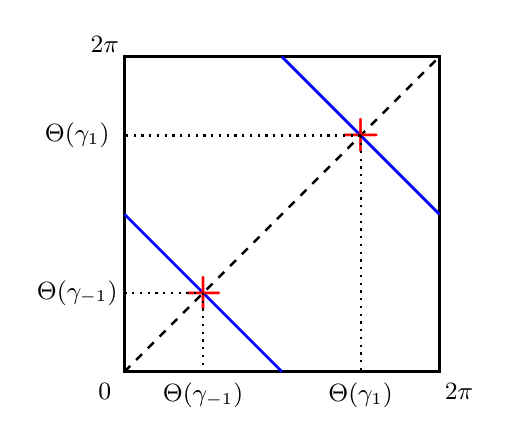
\begin{tikzpicture}[scale=1, every node/.style={font=\small}]
  \def\S{4.0} % side length of the square

  % square [0,1]^2 scaled by S
  \draw[line width=0.9pt] (0,0) rectangle (\S,\S);
    
  % the two diagonal segments (slope -1)
  \draw[blue, line width=1pt] (\S*0.5,0) -- (0,\S*0.5);
  \draw[blue, line width=1pt] (\S, \S*0.5) -- (\S*0.5,\S);

  % dashed diagonal
  \draw[dashed,line width=0.9pt] (0,0) -- (\S,\S);

  % the two X marks
  \node[text=red, font=\bfseries\boldmath, scale=1.6] at (\S*0.25,\S*0.25) {$+$};
  \node[text=red, font=\bfseries\boldmath, scale=1.6] at (\S*0.75,\S*0.75) {$+$};

  \draw[dotted, line width=0.8pt] (\S*0.25, \S*0.25) -- (\S*0.25, 0);
  \node at (\S*0.25,-0.3) {$\Theta(\gamma_{-1})$};
  \draw[dotted, line width=0.8pt] (0, \S*0.25) -- (\S*0.25, \S*0.25);
  \node at (-0.6,\S*0.25) {$\Theta(\gamma_{-1})$};
  \draw[dotted, line width=0.8pt] (\S*0.75, \S*0.75) -- (\S*0.75, 0);
  \node at (\S*0.75,-0.3) {$\Theta(\gamma_{1})$};
  \draw[dotted, line width=0.8pt] (\S*0.75, \S*0.75) -- (0, \S*0.75);
  \node at (-0.6,\S*0.75) {$\Theta(\gamma_{1})$};

  % corner labels 0 and 2pi like your sketch
  \node at (-0.25,-0.25) {$0$};
  \node at (\S+0.25,-0.25) {$2\pi$};
  \node at (-0.25,\S+0.15) {$2\pi$};

\end{tikzpicture}

    \caption{Endpoint path $\Lambda(t)$ on $T^2$.}
\end{figure}
\FloatBarrier

\noindent \textbf{Target Set Path on the Torus.} 
We now describe the subset of $T^2$ corresponding to curves that connect a vertex (respectively, an edge) to its opposite side:
\begin{itemize}
\item \emph{Odd $n$:} For each vertex $V_i$ with opposite side $E_{V_i}^{opp}$, the set
\[
\mathcal{R}_i := V_i\times E_{V_i}^{opp} \ \cup\ E_{V_i}^{opp}\times V_i
\]
is a line on $T^2$ representing endpoint pairs with one on $V_i$ and the other on $E_{V_i}^{opp}$.

\begin{figure}[ht]
    \centering
    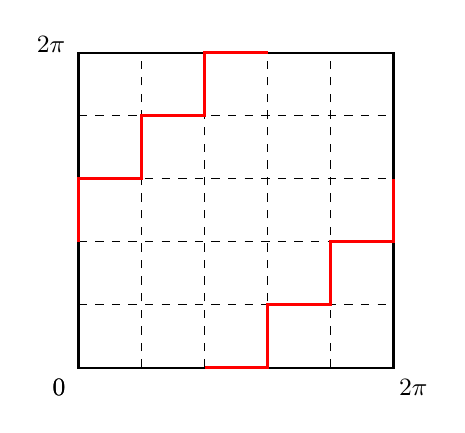
\begin{tikzpicture}[scale=1, every node/.style={font=\small}]
  \def\S{4} % side length of the square

  % --- draw outer square
  \draw[line width=0.9pt] (0,0) rectangle (\S,\S);

  % --- equally spaced dotted lines (4 each direction)
  \foreach \i in {1,2,3,4}{
    % verticals
    \draw[dashed] (\i*\S/5,0) -- (\i*\S/5,\S);
    % horizontals
    \draw[dashed] (0,\i*\S/5) -- (\S,\i*\S/5);
  }

  \draw[red,line width=1.2pt]
    (0,2*\S/5) -- (0,3*\S/5) -- (\S/5,3*\S/5) -- (\S/5,4*\S/5) --
    (2*\S/5,4*\S/5) -- (2*\S/5,5*\S/5) -- (3*\S/5,5*\S/5);
    
  \draw[red,line width=1.2pt]
    (2*\S/5,0) -- (3*\S/5,0) --
    (3*\S/5,\S/5) -- (4*\S/5,\S/5) -- (4*\S/5,2*\S/5) --
    (5*\S/5,2*\S/5) -- (5*\S/5,3*\S/5);

  % --- axis labels
  \node at (-0.25,-0.25) {$0$};
  \node at (\S+0.25,-0.25) {$2\pi$};
  \node at (-0.35,\S+0.1) {$2\pi$};
  \node at (-0.25,-0.25) {$0$};
\end{tikzpicture}
    \caption{The collection $\cup_{i=1}^n \mathcal R_i$ forming a closed “staircase” loop on $T^2$.}
\end{figure}
\FloatBarrier

\item \emph{Even $n$:} For each edge $E_i$ with opposite edge $E_{E_i}^{opp}$, the set
\[
\mathcal{R}_i := E_i\times E_{E_i}^{opp} \ \cup\ E_{E_i}^{opp}\times E_i
\]
is a rectangular patch on $T^2$ representing endpoint pairs with one on $E_i$ and the other on $E_{E_i}^{opp}$.
\begin{figure}[ht]
    \centering
    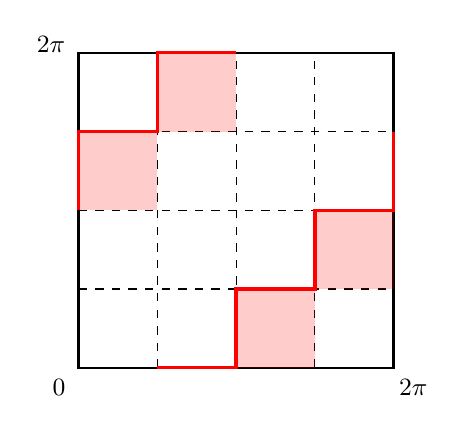
\begin{tikzpicture}[scale=1, every node/.style={font=\small}]
  \def\S{4.0} % side length of the square

  % --- outer square
  \draw[line width=0.9pt] (0,0) rectangle (\S,\S);

  % --- equally spaced dotted lines (3 each direction for 4x4 grid)
  \foreach \i in {1,2,3}{
    \draw[dashed] (\i*\S/4,0) -- (\i*\S/4,\S);   % vertical
    \draw[dashed] (0,\i*\S/4) -- (\S,\i*\S/4);   % horizontal
  }

  % --- staircase path (red) for 4x4 grid
  \fill[red,opacity=0.2] (0,2*\S/4) rectangle (\S/4,3*\S/4);
  \fill[red,opacity=0.2] (\S/4,3*\S/4) rectangle (2*\S/4,4*\S/4);
  \fill[red,opacity=0.2] (2*\S/4,0) rectangle (3*\S/4,\S/4);
  \fill[red,opacity=0.2] (3*\S/4,\S/4) rectangle (4*\S/4,2*\S/4);

  \draw[red,line width=1.2pt]
    (0,2*\S/4) -- (0,3*\S/4) -- (\S/4,3*\S/4) -- (\S/4,4*\S/4) --
    (2*\S/4,4*\S/4);

  \draw[red,line width=1.2pt]
    (\S/4,0) -- (2*\S/4,0) -- (2*\S/4,\S/4) -- (3*\S/4,\S/4) -- 
    (3*\S/4,2*\S/4) -- (4*\S/4,2*\S/4) -- (4*\S/4,3*\S/4);

  % --- axis labels
  \node at (-0.25,-0.25) {$0$};
  \node at (\S+0.25,-0.25) {$2\pi$};
  \node at (-0.35,\S+0.1) {$2\pi$};
\end{tikzpicture}

    \caption{The collection of $\{\mathcal{R}_i\}_{i=1}^n$ (shaded) and the subset of their union (solid red) which forms the closed  “staircase” loop.}
\end{figure}
\FloatBarrier
\end{itemize}
In either case, the union of these pieces, $\mathcal{R}:=\cup_{i=1}^n\mathcal{R}_i$ is connected and homologically nontrivial (cannot be contracted to a point). From this union we may select a single closed “staircase” path in $T^2=S^1 \times S^1$, which can be smoothed to a loop $R$ - the target set. Traversing $R$ once follows the counter-clockwise order of edges in both endpoint coordinates simultaneously, so it winds once around each $S^1$ factor in the same direction. Thus $R$ has homology class $[R]=(1,1)$, recording that as a point $x$ traverses $\partial P$ once clockwise, a point constrained to lie on the side opposite of $x$ also makes one clockwise circuit of the perimeter. \\

\noindent \textbf{Intersection argument.}
By Proposition (\ref{prop:AI-num-torus}), the algebraic intersection of $(p,q)$ and $(p',q')$ in $T^2$ is \(\widehat{i}((p,q),(p',q')) = pq'-p'q\). Substituting $[\Lambda]=(1,-1)$ and $[R]=(1,1)$ gives
\begin{align*}
\widehat{i}\big([\Lambda],[R]\big)=\widehat{i}\big((1,-1),(1,1)\big)=2\neq0.
\end{align*}
Since the intersection number is nonzero, $\Lambda$ and $R$ must intersect in $T^2$.

\noindent\textbf{Conclusion.}
An intersection point corresponds to some $t_0$ such that $(a_{t_0},b_{t_0})$ lies in one of the above sets, i.e.\ $\gamma_{t_0}$ has one endpoint on a vertex $V$ or an edge $E$ and the other on its opposite side, as claimed.
\end{proof}



\begin{theorem}[First width of convex polygons]\label{thm:first-width-convex-polygon}
For a compact convex polygon $P$ with $n$ sides, the first width is
\begin{equation}\label{eq:first-width-convex-polygons}
    \omega_1(P) = 
    \begin{cases}
        \displaystyle \min_{1\le i\le n}\ \operatorname{dist}\!\big(V_i,E_{V_i}^{\mathrm{opp}}\big), & \text{if $n$ is odd},\\
        \displaystyle \min_{1\le i\le n}\ \operatorname{dist}\!\big(E_i,E_{E_i}^{\mathrm{opp}}\big), & \text{if $n$ is even}.
    \end{cases}
\end{equation}
\end{theorem}

\begin{proof}
\textbf{Lower bound.} 
By Lemma~\ref{lem:polygon-width-ub}, for any sweep--out 
$\{\gamma_t\}_{t\in[-1,1]}$ of $P$ there exists $t_0$ such that:
\begin{itemize}
    \item if $n$ is odd, $\gamma_{t_0}$ joins some vertex $V_i$ to its opposite edge $E_{V_i}^{\mathrm{opp}}$;
    \item if $n$ is even, $\gamma_{t_0}$ joins some edge $E_i$ to its opposite edge $E_{E_i}^{\mathrm{opp}}$.
\end{itemize}
In either case, $\gamma_{t_0}$ has length at least the perpendicular distance between the relevant vertex/edge and its opposite edge. Therefore,
\[
\sup_{t} \mathrm{Length}(\gamma_t) \;\ge\;
\begin{cases}
    \displaystyle \min_{1\le i\le n} \operatorname{dist}\!\big(V_i,E_{V_i}^{\mathrm{opp}}\big), & \text{if $n$ is odd},\\[0.8em]
    \displaystyle \min_{1\le i\le n} \operatorname{dist}\!\big(E_i,E_{E_i}^{\mathrm{opp}}\big), & \text{if $n$ is even}.
\end{cases}
\]
Taking the infimum over all sweep--outs, we obtain
\[
\omega_1(P) \;\ge\;
\begin{cases}
    \displaystyle \min_{1\le i\le n} \operatorname{dist}\!\big(V_i,E_{V_i}^{\mathrm{opp}}\big), & \text{if $n$ is odd},\\[0.8em]
    \displaystyle \min_{1\le i\le n} \operatorname{dist}\!\big(E_i,E_{E_i}^{\mathrm{opp}}\big), & \text{if $n$ is even}.
\end{cases}
\]

\medskip
\noindent\textbf{Upper bound.} 
Let $A$ be a vertex (if $n$ is odd) or an edge (if $n$ is even) attaining the above minimum, and let $E_A^{\mathrm{opp}}$ be its opposite edge. Let $L$ be the supporting line of $P$, parallel to $E_A^{\mathrm{opp}}$, which passes through $A$ by convexity of $P$. Consider the sweep--out $\{\gamma_t^0\}_{t\in[-1,1]}$ obtained by intersecting $P$ with lines \emph{perpendicular} to $E_A^{\mathrm{opp}}$. Each curve $\gamma_t^0$ is perpendicular to both $L$ and $E_A^{\mathrm{opp}}$ and is contained between them, hence
\[
\mathrm{Length}(\gamma_t^0) \leq \operatorname{dist}(L,E_A^{\mathrm{opp}})
\quad \text{for all } t.
\]
Therefore
\[
\omega_1(P) \;\le\; \sup_t \mathrm{Length}(\gamma_t^0) 
= \operatorname{dist}(L,E_A^{\mathrm{opp}}),
\]
and by the choice of $A$ this equals the right-hand side of~\eqref{eq:first-width-convex-polygons}.

\noindent \textbf{Equality.} Combining the lower and upper bounds yields equality, as required.
\end{proof}